\section{Bio-Mechanical knee}

\subsection{Overview}
The work done in this section was in collaboration with Alex Tacescu \cite{tacescu2021development} and presented at International Mechanical Engineering Congress 2021 [WAITING FOR CITATION]. I led and managed the focus of the project and came up with the idea. I was also involved with running the mocap experiments and the mechanical design. Another knee design was examined that focused on matching the knee motion profile to a human knee. Exoskeletons discussed in \autoref{sec:ExoBack} commonly use pin-type joints in their knee joints; this is in contrast to how the actual kinematics work in a human knew, which has a variable center of rotation or a floating axis \cite{morrison1970mechanics} \cite{koo2008knee} \cite{grood1983joint}. This is illustrated by examining MRI scans of the knee, which show that the femur and tibia have oblong heads\cite{MRIKneeScan}. This geometry translates the tibia as the knee rotates. 


% \begin{figure}[h!]
%     \centering
%     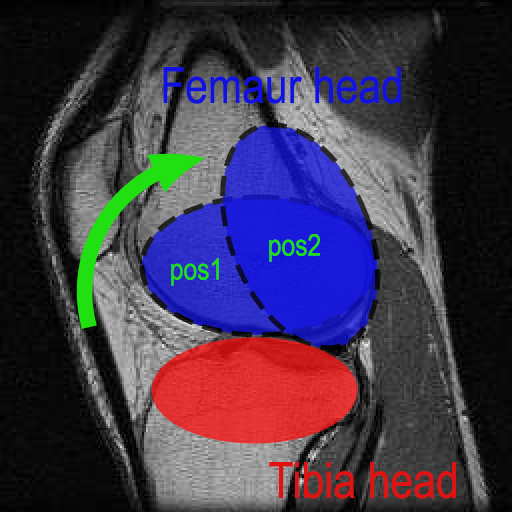
\includegraphics[scale=0.5]{images/mech_design/High-resolution-knee-scan-Resolution-is-025x025x15mm.png}
%     \caption[Labled MRI of knee]{MRI of knee the blue oval is the femur head and the red is the tibia head. as the knee rotates the shape of the femur head causes translate of the tibia. As shown in the two position of the femur head.}
%     \label{fig:MRIKnee}
% \end{figure}


\begin{figure}[h!]
    \centering
    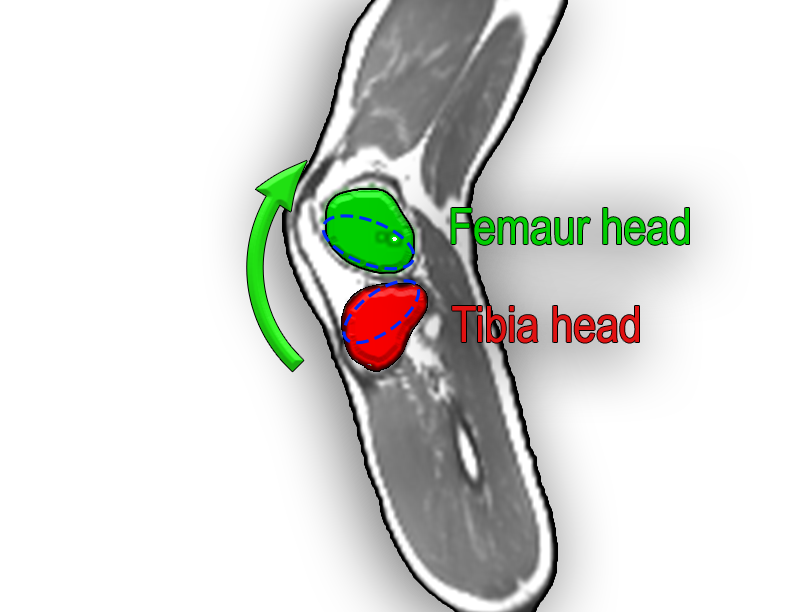
\includegraphics[scale=0.5]{images/mech_design/MRI_knee_label.png}
    \caption[Labled MRI of knee]{MRI of knee with the femur and tibia heads segmented and labeled. The heads of the joints can be approximated as ovals. }
    \label{fig:MRIKnee}
\end{figure}

Several recent designs have focused more on accounting for knee motion. Choi \textit{et. al} used multiple rolling cams to adapt to the changing center of rotation \cite{choi2017development}. This design fits a person's knee motion; it did not use modeling of the knee's tibiofemoral motion to design the cams. Additionally, the design is complicated and not easily reproducible. In another design Choi \textit{et. al} used multiple rollers and pulleys powered by electric linear actuators. However, rotary electric motors with rotary gearboxes can often achieve higher performance than electric linear actuators powered by rotary DC motors. Another knee design was presented in \cite{wang2018comfort}; this design prioritized the comfort of the user and the alignment of the knee joint. This design also uses pulleys and cables to model the knee motion. \cite{AdaptiveKneeJoint} presents a cam knee design that uses a model of the knee motion. This design is a significant improvement over previous designs that merely compensate for the motion. However, as the other designs discussed, they use linear actuators. These designs do well at either mimicking or compensating for the knee motion; however, they are mechanically cumbersome to manufacture; they did not show mimicking of the center of rotation's theoretical movement and/or use a linear actuator to replicate rotary motion. In addition, the design does not allow for the knee to be customized and therefore cannot meet the specific motion of the patient. Thus, we propose a knee design that is readily configured to match a particular patient's knee joint motion, is designed for easy manufacturing and allows the use of readily available rotary actuators and brake mechanisms.

The variable center of rotation was found using previous work by Iwaki \textit{et. al} that used Magnetic Resonance Imaging (MRI) scans to determine and predict the knee's trajectory \cite{MRIKneeShape_Loaded, MRIKneeShape_Unloaded}. These studies used cadavers and actual patients to measure the motion of the knee in both loaded and unloaded scenarios. This MRI data was used in \cite{KinDynKneeJoint} to build a mathematical model of knee motion that considers both the flexion and extension degrees of freedom. They used ellipse to model the contact between the femur and tibia bones. Their work leads to the formulation of \autoref{eq:KneeExtensionFlexionNumeric}. This equation relates the rotation (in radians) of the knee to the translation of the tibia. In these equation $a$ is a scaling factor and $d$ is an initial offset \cite{wang2013adaptive}. Both of these values are patient-specific and can be found using an MRI or motion capture study. This motion and its derivative are shown in \autoref{fig:FlexExtRelationship}. This study was limited since it was based on the anthropomorphic parameters of a single person. These coefficients will vary slightly from person to person and can be found using MRIs or potential motion capture. 

The difficulty in using motion capture is the error caused by manual palpation of bony landmarks and skin movement. The manual palpation of body land markers varies subject to subject and is difficult to be consistent. Several studies examined the effects of using skin markers to locate the floating knee axis, which can be on the order of several millimeters Eugene \textit{et. al} discussed several methods that decrease the skin movement error. \cite{alexander2001correcting} \cite{cappozzo1996position}. While these methods decrease the skin error, they are still not perfect, especially when examining the knee joint. Anderson \textit{et. al} found that even the addition of joint constraints did not improve the reliability of skin-mounted markers. Manipulation can also affect the accuracy of MRI knee studies; incorrectly identifying the correct body landmarks can affect kinematics studies and the location of the knee axis \cite{lerner2003use} and can result in 1.2mm or error. 


\begin{equation}
    r(\theta) mm = a(1.08\theta^4 - 11.18\theta^3 + 26.52\theta^2 - 0.825\theta) + d
    \label{eq:KneeExtensionFlexionNumeric}
\end{equation}



% \begin{figure}[ht!]
%     \centering
%     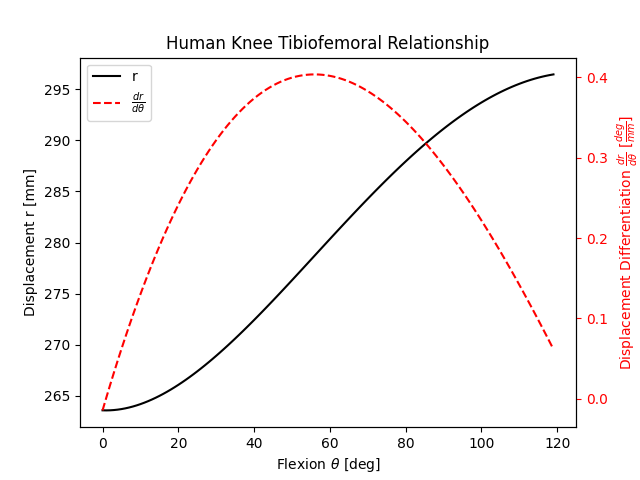
\includegraphics[scale=0.9]{images/mech_design/FlexionCurve.png}
%     \caption{Knee Flexion Curve}{Graphical representation of \autoref{eq:KneeExtensionFlexionNumeric} demonstrating the relationship between flexion and extension in a knee as measured by \cite{KinDynKneeJoint}. \(r(m)\) is the extension distance between the center of the knee and the center of mass of the lower leg. $0^\circ$ represents a perfectly extended knee joint.}
%     \label{fig:FlexExtRelationship}
% \end{figure} 


\subsection{Mechanical Development}

A cam-type mechanism with a brushless DC motor was designed to follow the desired path. The guide was generated using \autoref{eq:KneeExtensionFlexionNumeric}. 


\begin{figure}[ht!]
    \centering
    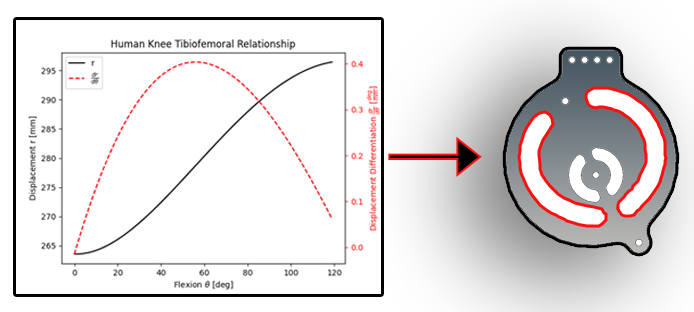
\includegraphics[scale=0.9]{images/mech_design/knee_plate_main_annotated.png}
    \caption{Knee Flexion Curve}{Graphical representation of \autoref{eq:KneeExtensionFlexionNumeric} demonstrating the relationship between flexion and extension in a knee as measured by \cite{KinDynKneeJoint}. \(r(m)\) is the extension distance between the center of the knee and the center of mass of the lower leg. $0^\circ$ represents a perfectly extended knee joint. The curve effects the shape of the red cam on the knee plate. }
    \label{fig:FlexExtRelationship}
\end{figure} 


\autoref{fig:a_varying} shows the effect of varying the scaling parameters. These values will scale the trajectory, affecting the relationship of the rotation and translation of the tibia. \autoref{fig:KneePlateDesign} shows the knee cam for several scaling values as illustrated it the cam profile is altered. This guide enforces variable center of rotation and motion of the tibia. \autoref{fig:ExplodedViewLabeled} shows an exploded view of the knee mechanism. 

\begin{figure}
    \centering
    \begin{subfigure}{\columnwidth}
        \centering
        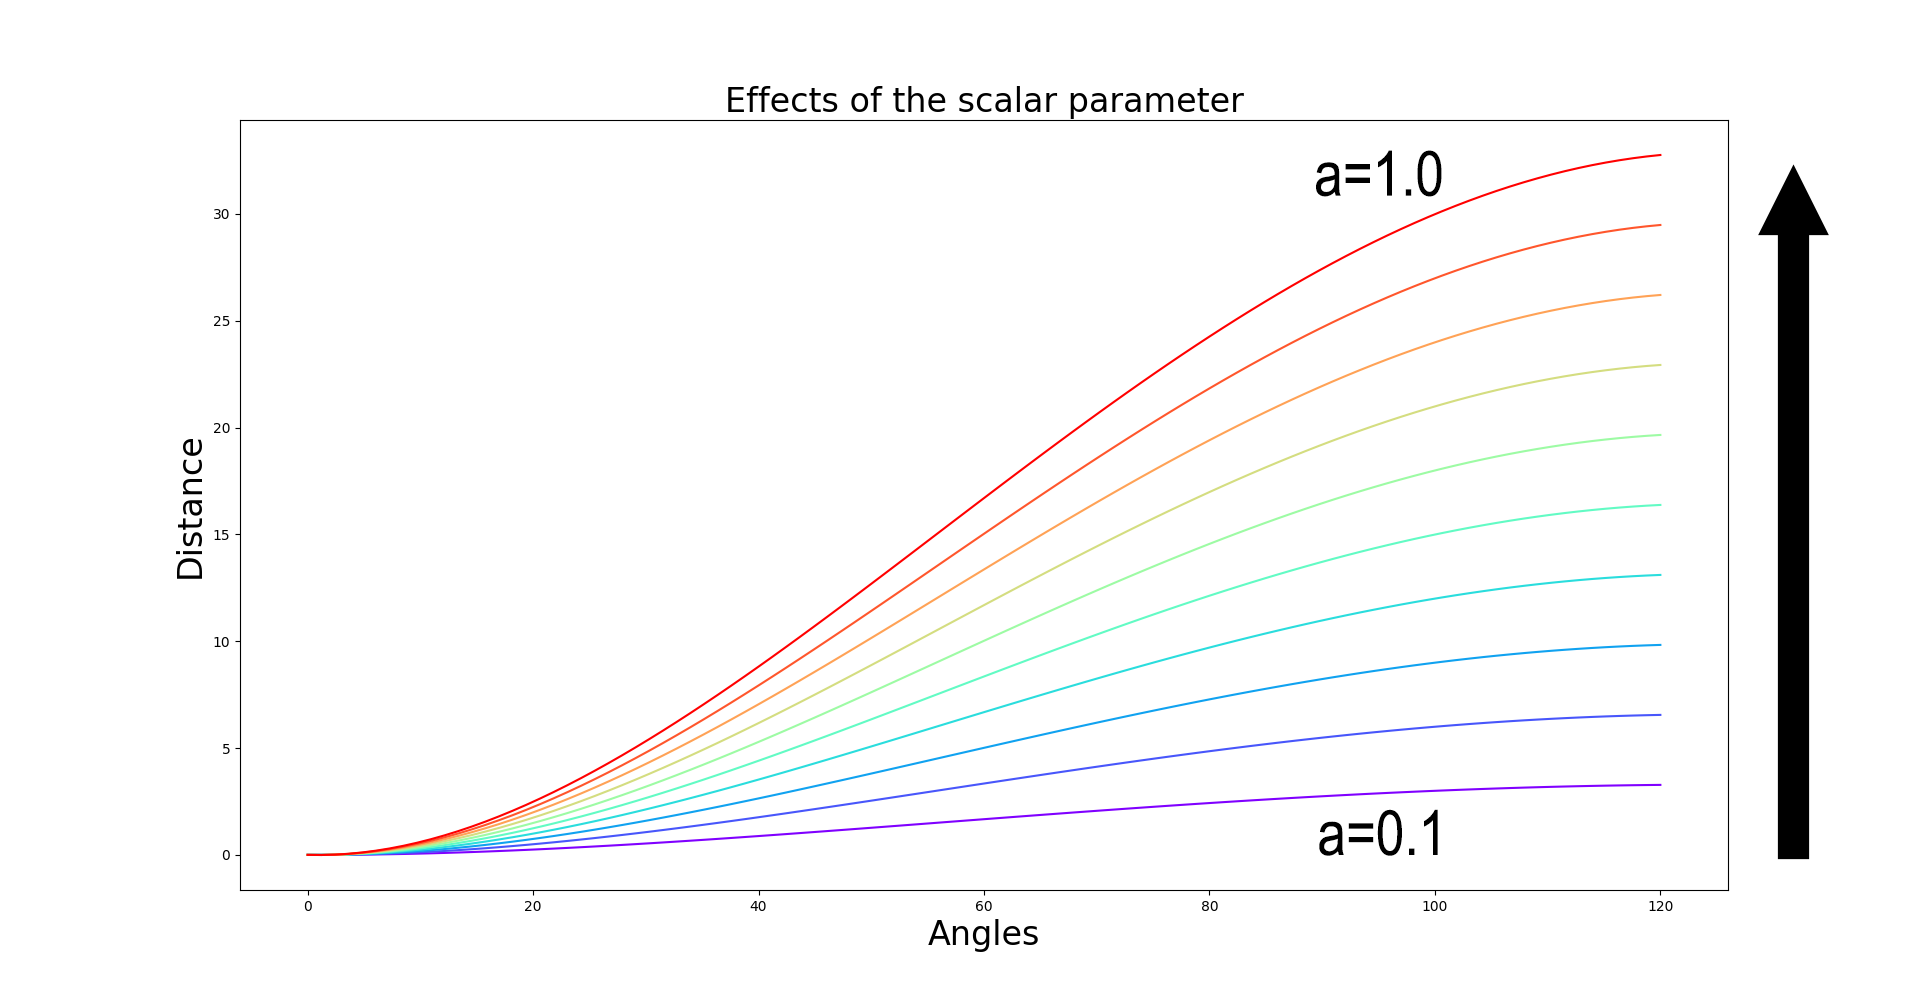
\includegraphics[width=\columnwidth]{images/mech_design/scalar_varying_a_Annotated.png}
        \caption[Scaling Parameter]{Varying the scaling parameter in \autoref{eq:KneeExtensionFlexionNumeric}. As the value of $a$ increase the angle vs. distance increases. Each line is a increase of $0.1$ starting at $a=0.1$ and ending at $a=1.0$.}
        \label{fig:a_varying}
    \end{subfigure}
    \begin{subfigure}{\columnwidth}
        \centering
        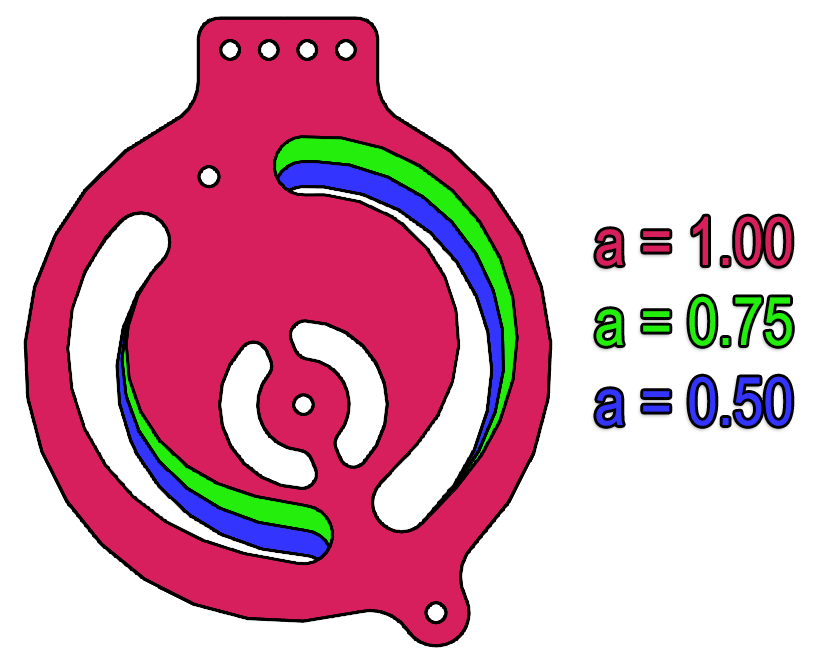
\includegraphics[scale=0.35]{images/mech_design/knee_model.png}
        \caption[Comparison of the Knee Cam]{Comparison of the knee cam as the scaling parameter is varied.}
        \label{fig:KneePlateDesign}
    \end{subfigure}
    \caption[Modular Knee Cam]{Modular Knee Cam, as the scaling parameter is altered the cam path also changes to meet the rotational \rightarrow transnational relationship.}
    \label{fig:kneecam}
\end{figure}








\begin{figure}
    \begin{subfigure}{\textwidth}
        \centering
        \captionsetup{justification=centering}
        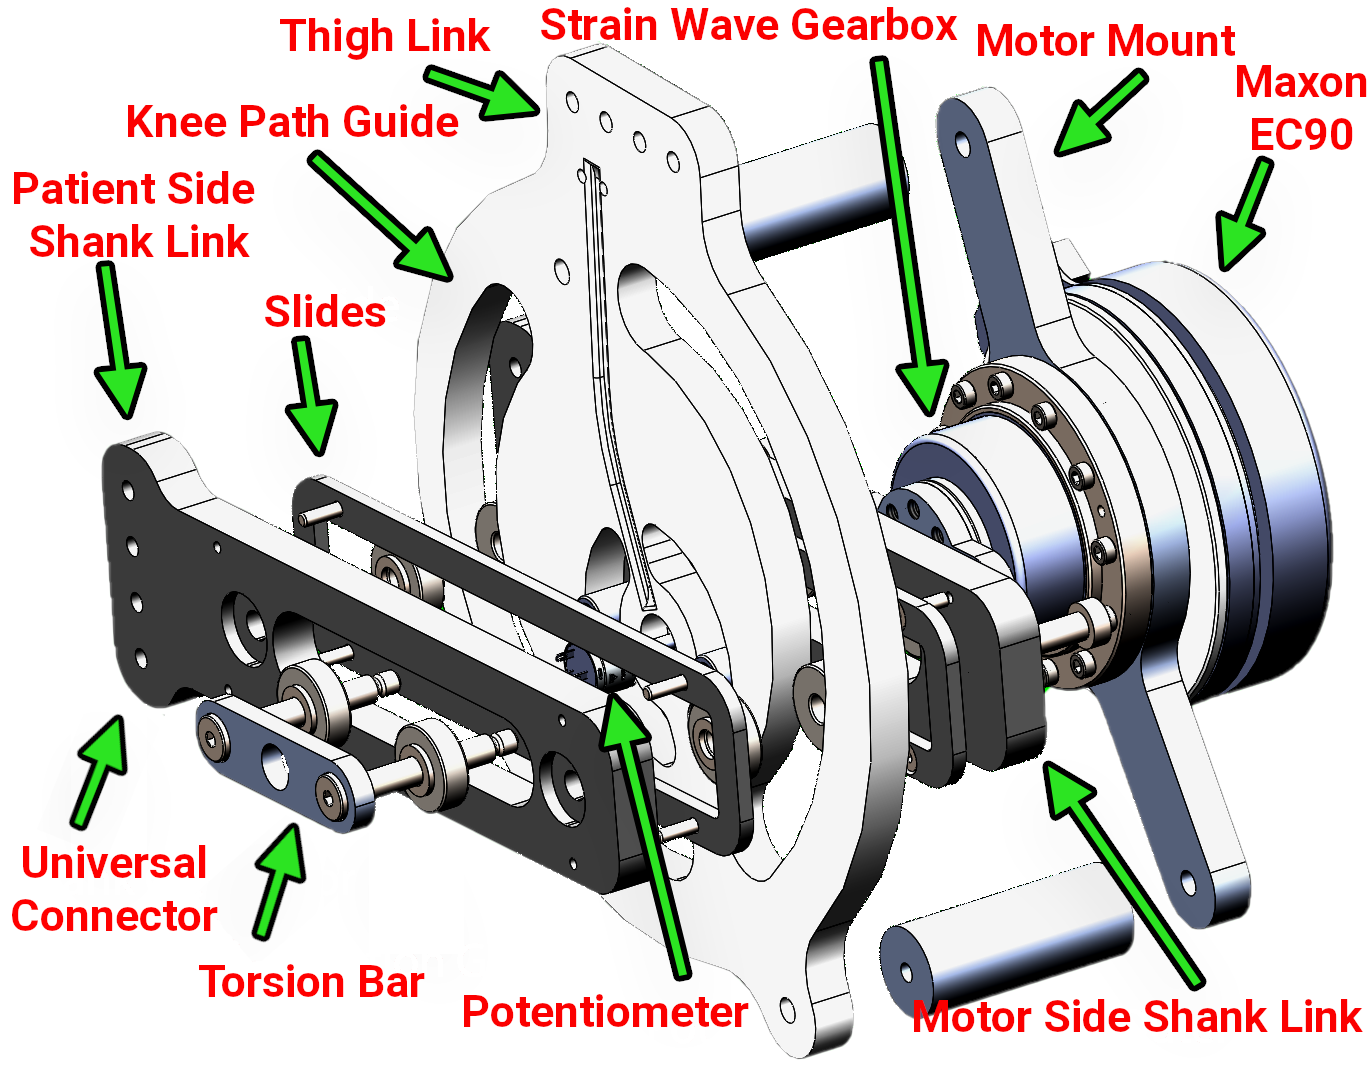
\includegraphics[scale=0.2]{images/mech_design/ExoKneeExplodedView.png}
        \caption{Bio Knee joint design exploded view}{Knee joint design exploded view}
        \label{fig:ExplodedViewLabeled}
    \end{subfigure}
    \begin{subfigure}{\textwidth}
        \centering
         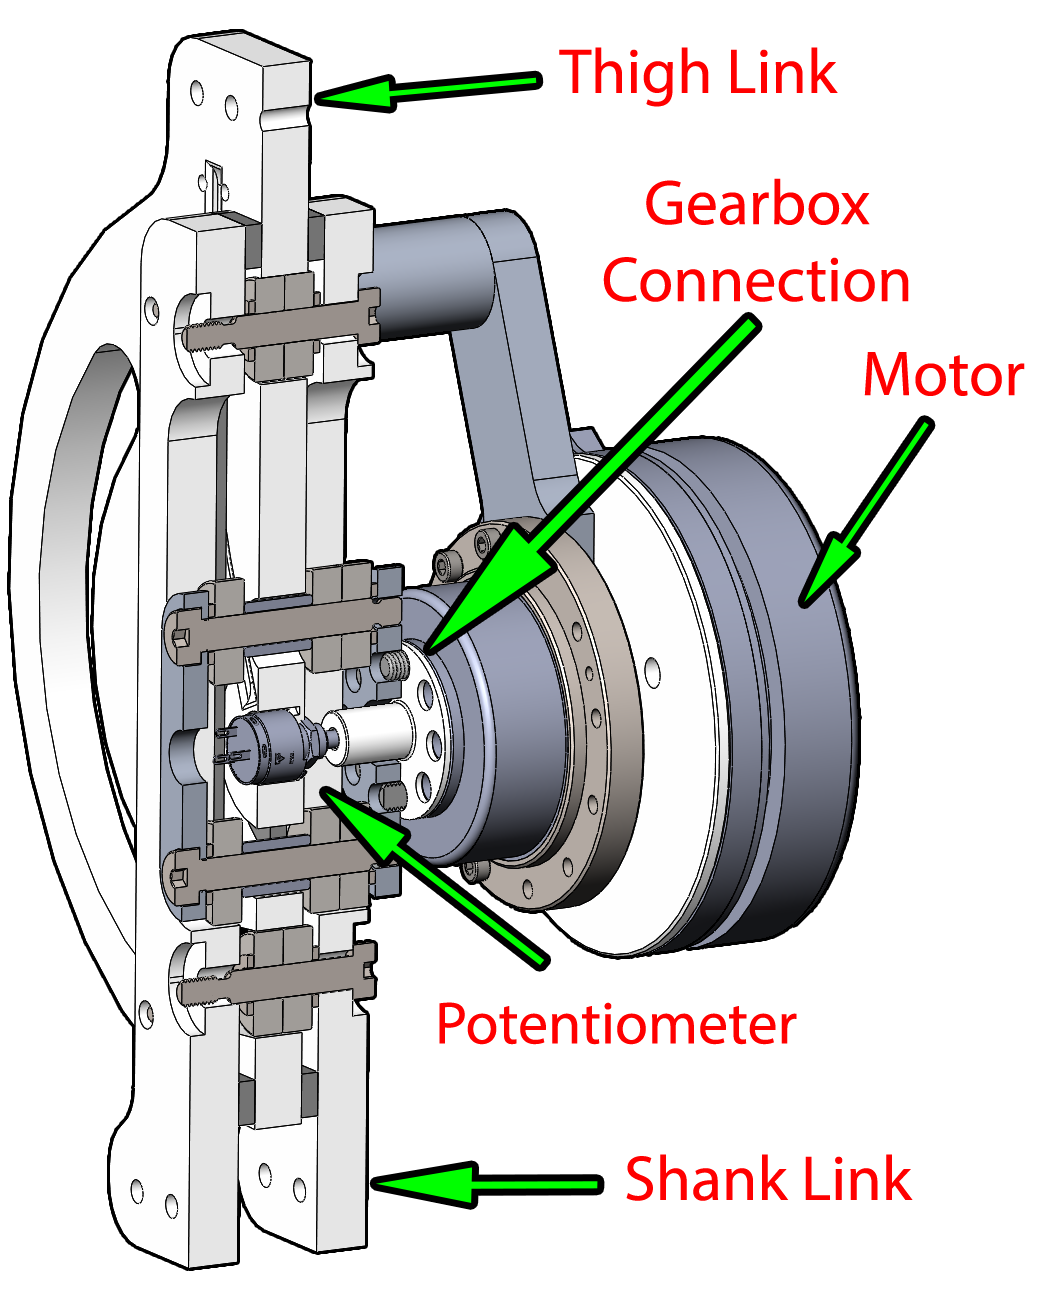
\includegraphics[scale=0.2]{images/mech_design/KneeJointAssyCrossSection.png}
          \captionsetup{justification=centering}
        \caption{Cross section of Bio knee}{A cross section of the knee joint with the potentiometer embedded in the design. The wires are routed along the wire channel to avoid interference with the inner arm and plastic slides}
        \label{fig:CrossSectionPot}
    \end{subfigure}    
    \caption{Exploded View of bio-knee mechanism}
    \label{fig:bioknee}
\end{figure}

The motor and gearbox need to provide sufficient torque and power to drive the knee of a $100kg$ patient through gait motion. This mass is larger than the average mass of the North American paraplegic, which is $68.8kg$, so assuming a larger mass allows for the motor to have a safety factor. Additionally, it is assumed that the dynamic loads are assumed to be negligible during the slow-motion collision with the ground. It equates to approximately $65W$ of power and $25Nm$ of torque at \(15^\circ/sec\). The knee is powered by a $90W$ brushless Maxon motor used with a nominal torque of $0.56Nm$ at roughly $2500rpm$. The motor is combined with a Harmonic gearbox with a $100:1$ reduction. \autoref{table:MotorGearboxSpecs} shows the gearbox and motor specifications and the joint's mechanical properties. As per the manufacturer documentation, the calculations assumed an efficiency of \(90\%\). The designed knee joint can mechanically output $81W$ and $50.4Nm$ at $15^\circ/sec$.  

\begin{table}
    \centering
    \begin{tabular}{||c|c|c||}
        \hline
        Input (Motor) Power & \(P_{input}\) & \(90 Watts\) \\
        \hline
        Input (Motor) Torque @ Nominal & \(\tau_{input}\) & \(0.560 Nm\) \\
        \hline
        Input (Motor) Speed @ Nominal & \(\omega_{input}\) & \(2510 rpm\) \\
        \hline
        Input (Motor) Stall Torque & \(\tau_{in\_stall}\) & \(7.480 Nm\) \\
        \hline \hline
        Gearbox Ratio & \(\frac{n_1}{n_2}\) & \(100:1\) \\
        \hline \hline
        Output Power & \(P_{output}\) & \(81 Watts\) \\
        \hline
        Output Torque @ Nominal & \(\tau_{input}\) & \(50.4 Nm\) \\
        \hline
        Output Speed @ Nominal & \(\omega_{input}\) & \(15^\circ/sec\) \\
        \hline
        Output Stall Torque & \(\tau_{out\_stall}\) & \(673.2 Nm\) \\
        \hline
    \end{tabular}
    \caption{Bio Knee parameters}{Motor/gearbox specifications and output power specifications of the proposed joint.}
    \label{table:MotorGearboxSpecs}
\end{table}

\subsection{Design Analysis}

The design was validated using a motion capture system and SolidWorks motion analysis \footnote{https://www.solidworks.com/category/simulation-solutions}. The markers on the knee were aligned on the shank and thigh segments of the knee and rotated through the desired motion as shown in \autoref{fig:KneeJointTestSetup}; this allowed us to compare the theoretical trajectory to the actual trajectory, and for the measurement and comparison of manufacturing tolerance. \autoref{fig:KneeJointTestResults} shows the results of the study. There are some slight deviations of the actual motion compared to the desired motion; this deviation is caused by hysteresis in the system. However, these movements are very slight on a scale of less than $1mm$, which is assumed to be negligible.   



\begin{figure}[ht!]
    \centering
    \includegraphics[scale=0.07]{images/mech_design/KneeTrajTest_edit.png}
    \caption{Knee with mocap markers}{Knee joint setup with motion capture dots. The knee was manual rotated to measure the angle vs. distance relationship.}
    \label{fig:KneeJointTestSetup}
\end{figure}

\begin{figure}[ht!]
    \centering
    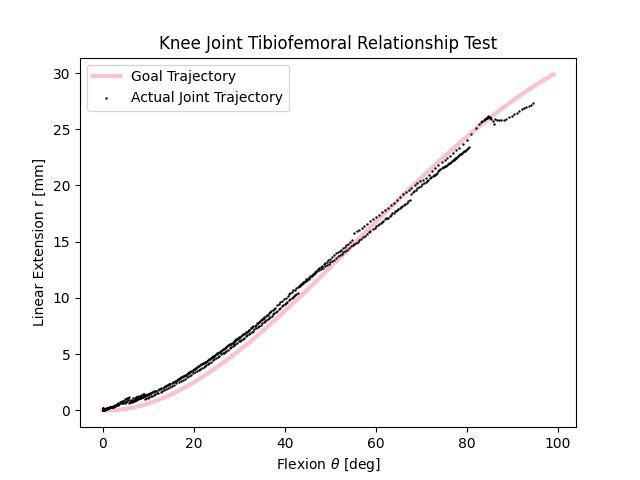
\includegraphics[scale=0.75]{images/mech_design/FlexionExtensionKneeJoint.png}
    \caption{Comparison of variable center of rotation}{Graph showing knee joint flexion vs linear extension of the radius of curvature for the goal trajectory (see \autoref{eq:KneeExtensionFlexionNumeric}) and the experimental results from the Motion Capture Study}
    \label{fig:KneeJointTestResults}
\end{figure}




\subsection{MRI Testing}

The work in this section is still under work and being done with Tess Meier. 


An MRI analysis was conducted to measure the bio joint's alignment with the underlying bone structure. The Worcester Polytechnic Institute IRB approved this study. In this study, 6 subjects were scanned in the MRI wearing a simple pin joint and the bio joint described above. Both joints were altered to be MRI compatible, which meant removing any metal in the joints. The pin joint knee is shown in \autoref{fig:MRIPINJoint} and the MRI compatible bio-joint is shown in \autoref{fig:MRIBIOJoint}. This alteration consisted of using only plastic nuts and bolts, the main cam body was water cut from polycarbonate, and the strap carriages were made from 3D printed PLA. A small piece of medical-grade foam was placed inside each strap carriage for patient comfort.    


\begin{figure}
    \begin{subfigure}{\textwidth}
        \centering
        \captionsetup{justification=centering}
        \includegraphics[width=0.75\linewidth]{images/mech_design/MRI_pinjoint.png}
        \caption{MRI compatible Pin-Joint}{MRI compatible pin joint with adjustable straps.  }
        \label{fig:MRIPINJoint}
    \end{subfigure}
    \begin{subfigure}{\textwidth}
        \centering
        \includegraphics[width=0.75\linewidth]{images/mech_design/MRI_bioknee.png}
          \captionsetup{justification=centering}
        \caption{MRI compatible Bio-Joint}{MRI compatible bio-joint with adjustable strap arms.}
        \label{fig:MRIBIOJoint}
    \end{subfigure}    
            \begin{subfigure}{\textwidth}
        \centering
        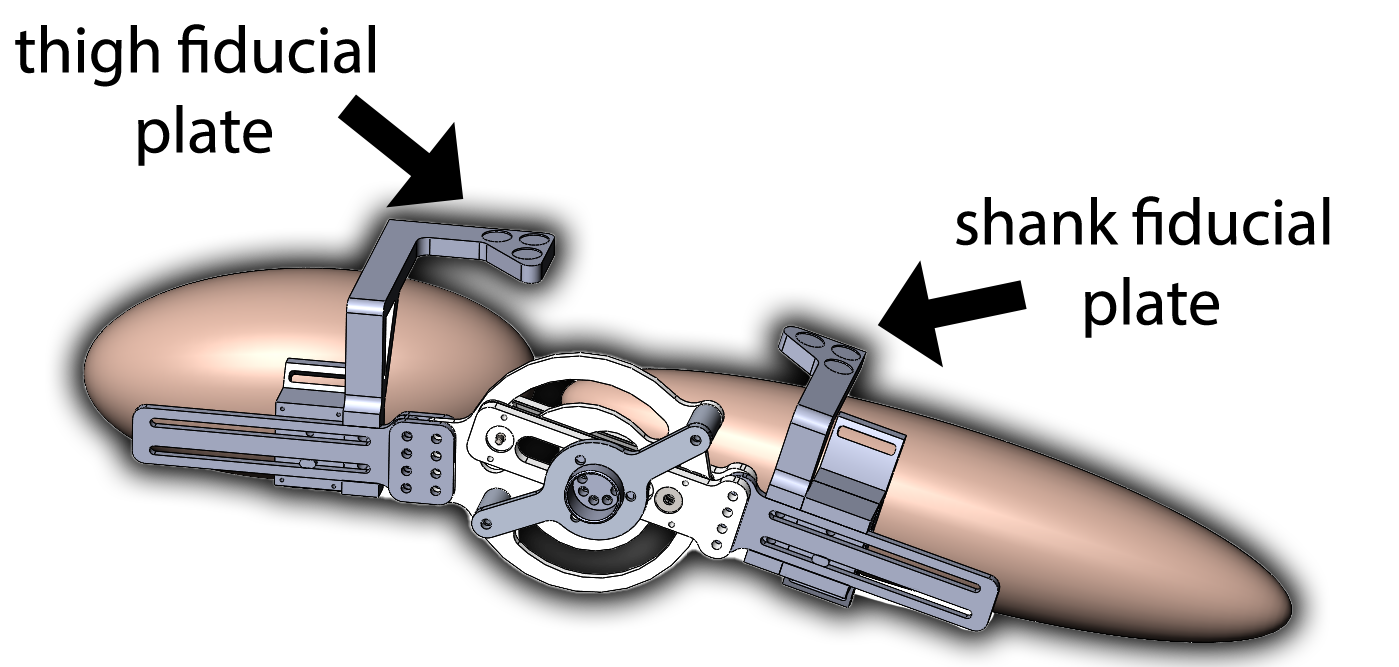
\includegraphics[width=0.75\linewidth]{images/mech_design/mri_knee_with_markers_edit.png}
          \captionsetup{justification=centering}
        \caption[fiducial stand off]{Fiducial stand offs brackets for MRI scans. The bracket move the segment markers closer together and towards the center of the bore.}
        \label{fig:MRIMarkerStandoff}
    \end{subfigure}
    \caption[MRI Compatible Knees]{MRI compatible knees made from PLA and polycarbonate. This device is made from polycarbonate and plastic bolts. The strap carriages can be adjusted in the channels to fit to the subject.}
    \label{fig:MRIKnees}
\end{figure}



In the study, the subjects were scanned wearing both the pin and bio joint at three different angles, the knee straight out ($0^{\circ}$), a high flex angle ($\sim34^{\circ}$),  and a mid-flex angle  ($\sim20^{\circ}$). \autoref{fig:MRIKneeAngles} shows an overlay of several MRI scans at different angles. This figure also illustrates the rolling-sliding motion of the femur head on the tibia head. 

A major obstacle in recording the scan was aligning the field of view with the fiducials on the joint. The diameter size of the bore prevented large angles from being measured. The bore diameter combined with the coil placement proved to be a significant challenge for the study. The limited field of view of the MRI made it challenging to locate the fiducials on the thigh and shank segments. The image would be distorted, or one or more fiducials was not captured. Additionally, the coil weight would push down on the bio knee, causing the device to rotate slightly. This unnatural rotation would effective the reliability of the data. To solve this problem, marker standoffs were created to move the markers closer together and closer to the center of the MRI scanner bore. \autoref{fig:MRIMarkerStandoff} shows a rendering of the fiducial standoffs. They were 3D printed and bolted to the arms of both knees. Foam blocks were placed under the subject's knee, and a foot brace was used to hold the position of the knee during the scan. Additionally, the foam was shaped for the different knee angles to lift the coil away from the joint; this prevented the coil from pressing down on the joint, causing the joint to rotate and become misaligned. 


\begin{figure}
    \centering
    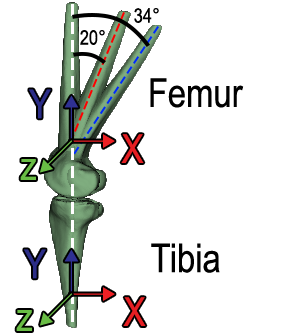
\includegraphics{images/mech_design/mri_knee_angles.png}
    \caption{MRI Knee Angles}{MRI scan of the femur and tibia overlayed from several scans taken at different knee angles. The coordinate frame for each of the bones and the measured angles are shown.}
    \label{fig:MRIKneeAngles}
\end{figure}


\begin{figure}
    \begin{subfigure}{\textwidth}
        \centering
        \captionsetup{justification=centering}
        \includegraphics[width=0.75\linewidth]{images/mech_design/wearing_MRI_pinjoint.png}
        \caption[Pin Joint in MRI ]{Subject wearing the pin joint in the MRI scanner.}
        \label{fig:MRIPINJoint}
    \end{subfigure}
    \begin{subfigure}{\textwidth}
        \centering
        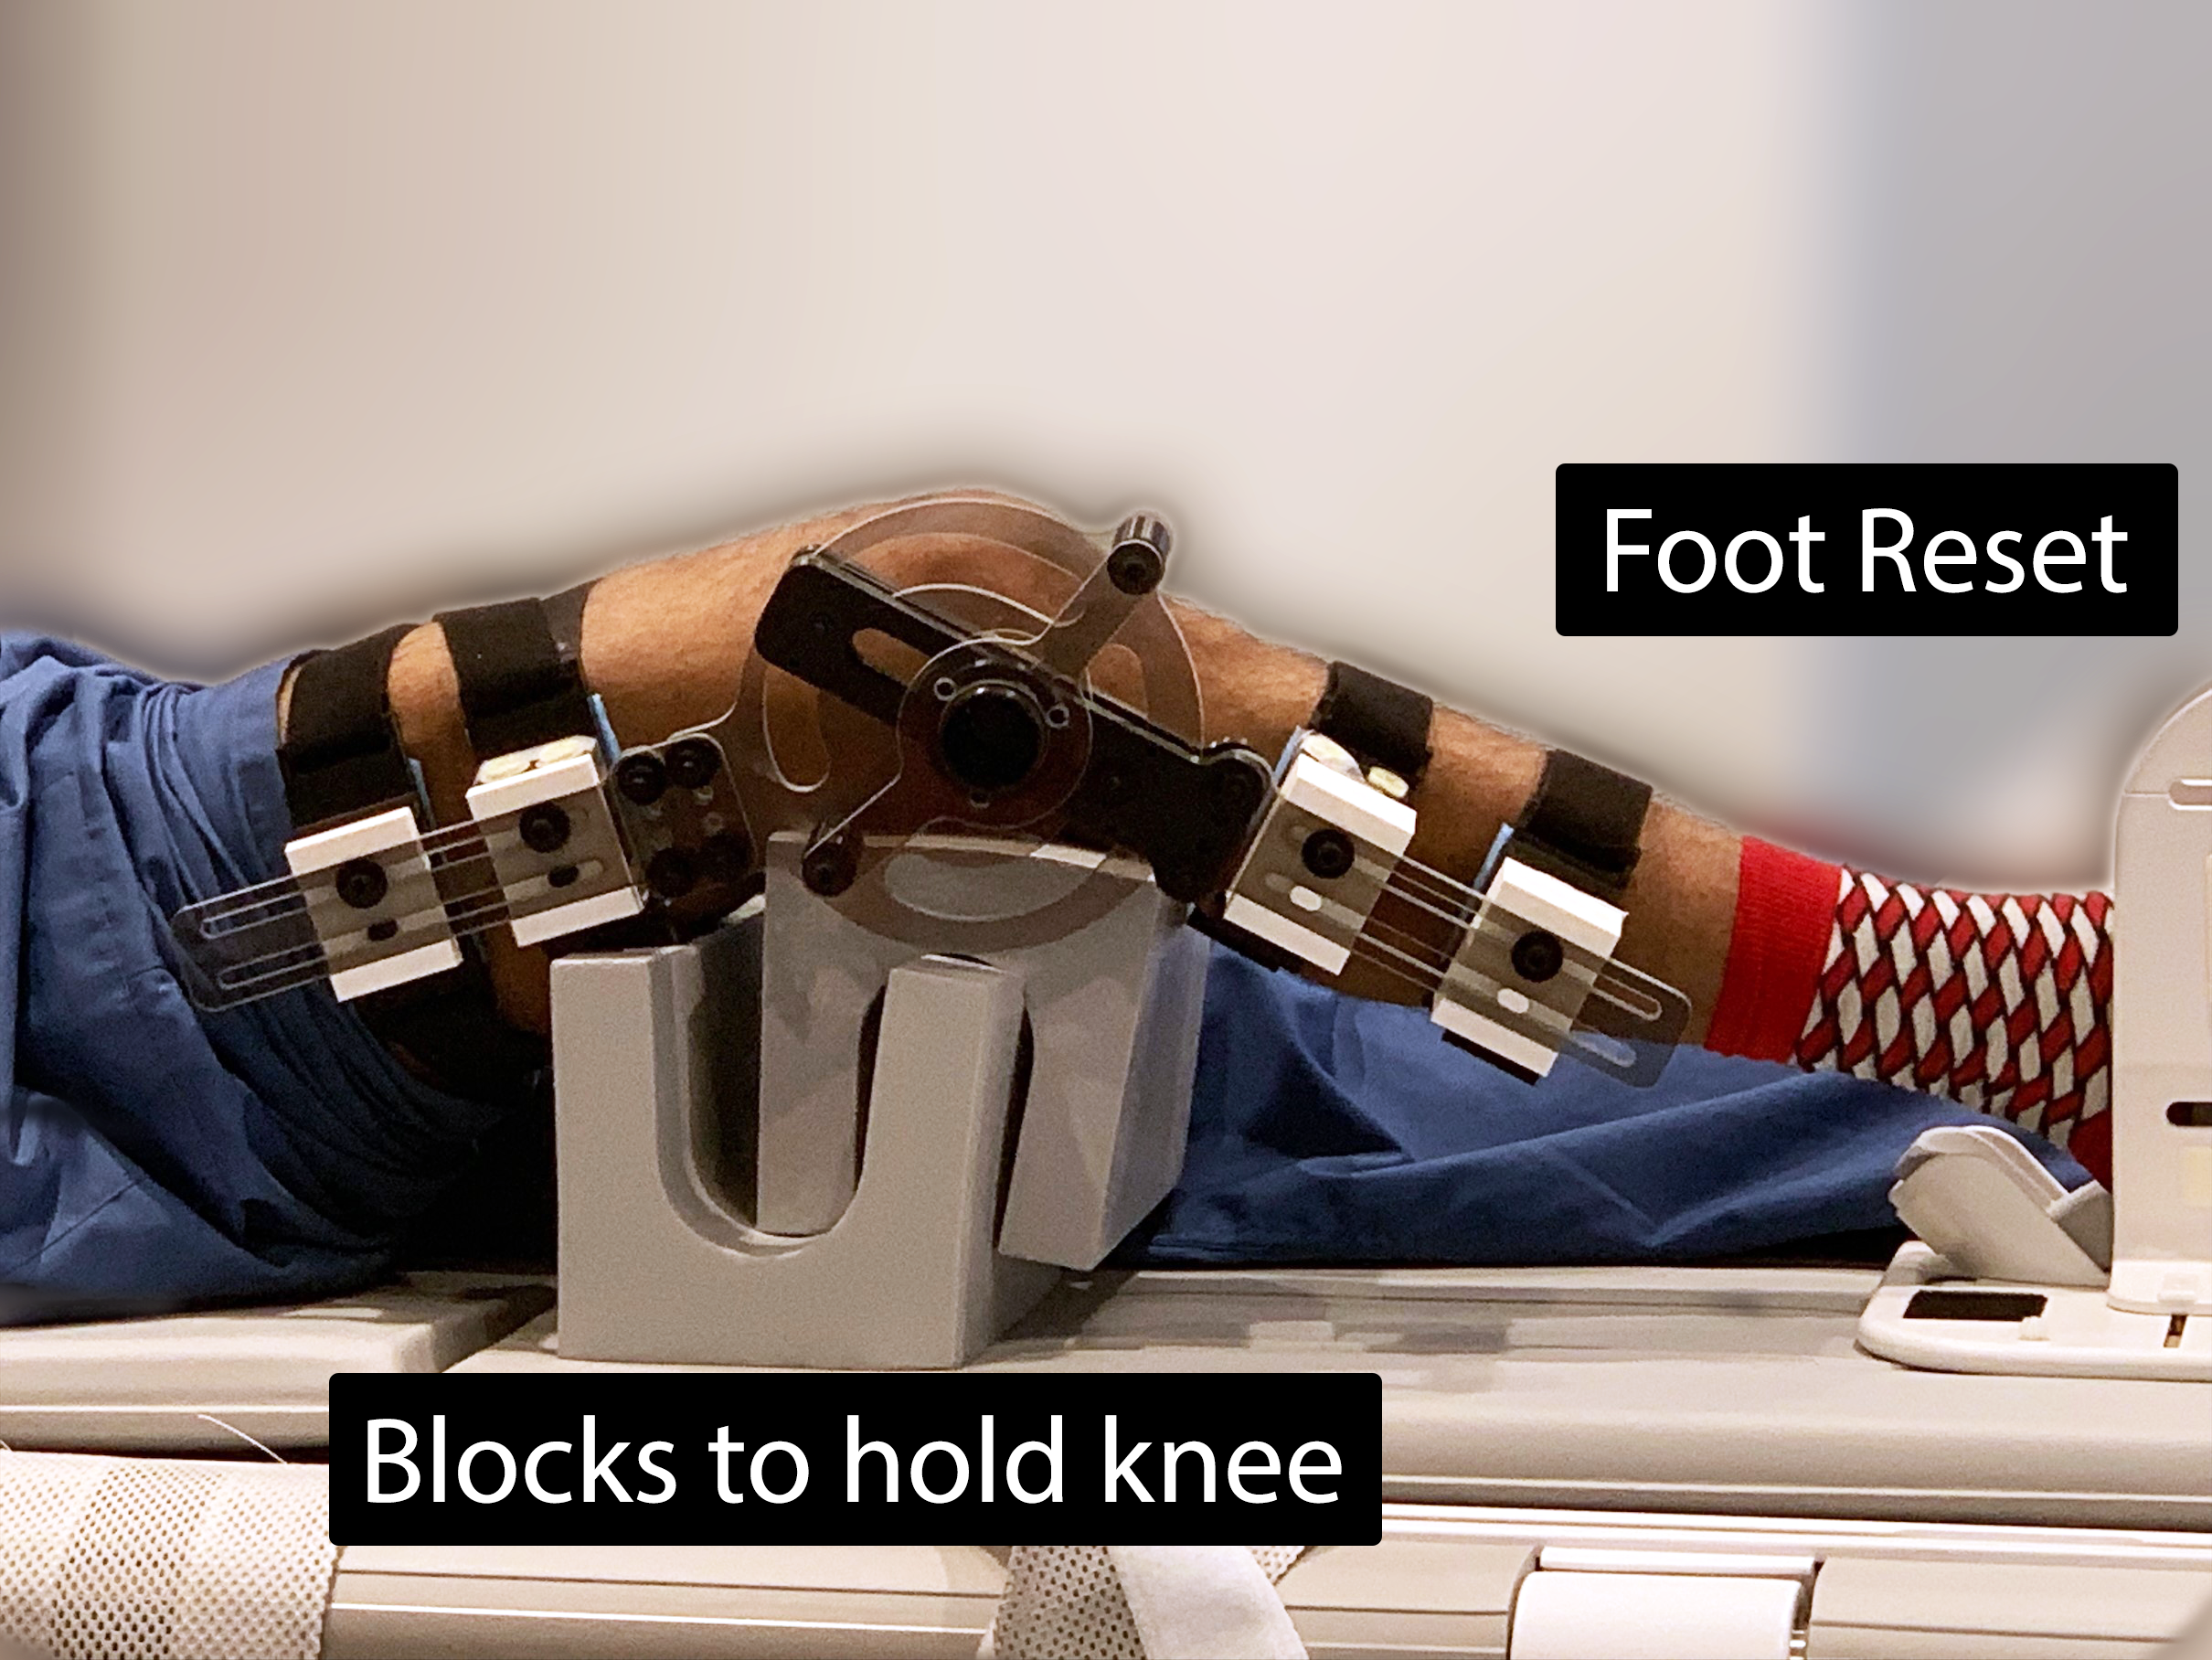
\includegraphics[width=0.75\linewidth]{images/mech_design/wearing_MRI_bioknee.png}
          \captionsetup{justification=centering}
        \caption[Bio-joint in MRI]{Subject wearing the bio-joint in the MRI scanner.}
        \label{fig:MRIBIOJoint}
    \end{subfigure}

    \caption{Subject wearing the MRI compatible joints in the MRI scanner.}
    \label{fig:MRIKnees}
\end{figure}


  



\section{Conclusion}
The presented prototype of the knee joint can move through the desired joint range and replicate the tibiofemoral path of a biological knee. \autoref{fig:LARRBio-Knee} shows the presented knee in the rendering of LARRE. The motor produces the required torque, and the potentiometer and encoder in the motor allow for feedback control. The use of FEA showed that the knee could withstand the anticipated forces without structurally failing. These tests are necessary for ensuring that the knee can withstand force. The knee is a key joint for maintaining upright posture and preventing falling. If the knee joint fails during operation, the patient could fall and be injured. 

A key part of the design was ensuring that the system could be easily manufactured and customized. All of the parts can be manufactured with minimal manufacturing experience and all of the custom components are 3D printable on inexpensive consumer-grade 3D printers with consumer-grade PLA filament. The other components are off-the-shelf components. The presented design is ideal for customization and manufacturing. The presented knee was designed to follow a previously established trajectory. Additional testing needs to be conducted to identify the patient-specific parameters so that the polynomial can be fitted to the individual. THIS WORK IS CURRENTLY ONGOING using MRI images of the femur and tibia heads or potential motion capture to measure the translation and rotation of the tibia relative to the femur. 

\begin{figure}
    \centering
    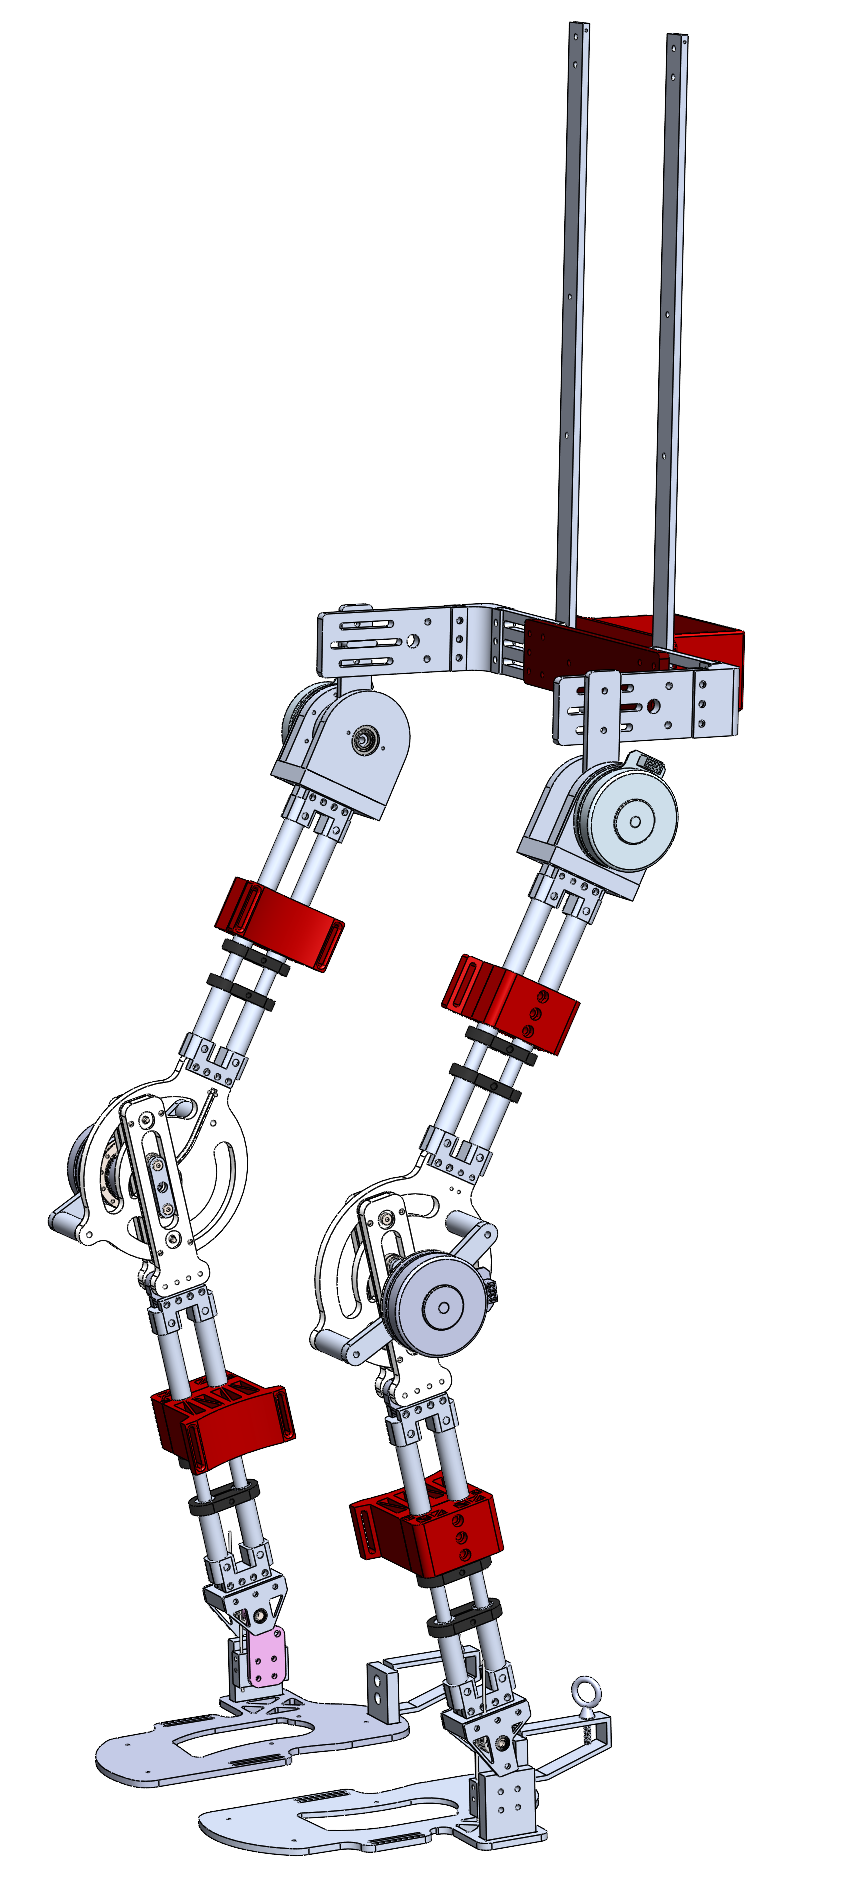
\includegraphics[scale=0.15]{images/mech_design/exo_with_bioknee.png}
    \caption[Rendering of LARRE with the Bio-Knee]{A Rendering of LARRE with the Bio-knee}
    \label{fig:LARRBio-Knee}
\end{figure}
